\documentclass[a4paper, 11pt]{article}
%\usepackage{qtree} %z jakiegoś dziwacznego powodu ten pakiet musi być aż tak wysoko...
\usepackage[OT4,plmath,MeX]{polski}
\usepackage{amstext, amsopn, amsfonts, amsthm, amsbsy, latexsym, amssymb}
\usepackage[utf8]{inputenc}

\usepackage{indentfirst}
\usepackage[margin=2cm]{geometry}
\usepackage{amsmath} %found in http://en.wikibooks.org/wiki/LaTeX/Formatting
\usepackage{amsfonts}
\usepackage{amssymb}
\usepackage{enumerate}
\usepackage{textcomp}

\usepackage{multirow}

\usepackage{graphicx}
\usepackage{epstopdf}
\usepackage{url}
\usepackage{hyperref}
\usepackage{multirow}
\usepackage{listings}

\newcommand{\HRule}{\rule{\linewidth}{0.5mm}}

\begin{document}

\begin{titlepage}
\begin{center}

% Upper part of the page. The '~' is needed because \\
% only works if a paragraph has started.

\includegraphics[width=0.15\textwidth]{./include/agh-logo}~\\[1cm]

\textsc{\LARGE Akademia Górniczo-Hutnicza w Krakowie}\\
\textsc{\Large Wydział Elektrotechniki, Automatyki, Informatyki i Inżynierii Biomedycznej}\\
[1.5cm]

\textsc{\Large Projekt zaliczeniowy}\\[0.5cm]

% Title
\HRule \\[0.4cm]
{ \huge \bfseries Analizator EKG}\\[0.4cm]

\HRule \\[1.5cm]

% Author and supervisor
\begin{minipage}{0.27\textwidth}
\begin{flushleft} \large
\emph{Autorzy:}\\
 Mateusz \textsc{Baran} \\
 Krzysztof \textsc{Bębenek} \\
 Bartłomiej \textsc{Bułat} \\
 Szczepan \textsc{Czaicki} \\
 Tomasz \textsc{Drzewiecki} \\
 Krzysztof \textsc{Farganus} \\
 Łukasz \textsc{Jaromi} \\
 Mateusz \textsc{Krasucki} \\
 Łukasz \textsc{Krzyżek} \\
 Łukasz \textsc{Kutrzuba} \\
 Weronika \textsc{Łabaj} \\
 Paweł \textsc{Maślanka} \\
\end{flushleft}
\end{minipage}
\begin{minipage}{0.27\textwidth}
\begin{flushleft} \large
 \phantom{Autorzy:}
 Piotr \textsc{Matuszkiewicz} \\
 Norbert \textsc{Pabian} \\
 Łukasz \textsc{Pękala} \\
 Krzysztof \textsc{Piekutowski} \\
 Grzegorz \textsc{Pietrzyk} \\
 Łukasz \textsc{Podolski} \\
 Mikołaj \textsc{Rzepka} \\
 Agata \textsc{Sitnik} \\
 Leszek \textsc{Sosnowski} \\
 Aleksander \textsc{Steliga} \\
 Mateusz \textsc{Ślażyński} \\
 Łukasz \textsc{Zieńkowski}
\end{flushleft}
\end{minipage}
\begin{minipage}{0.4\textwidth}
\begin{flushright} \large
\emph{Opiekun:} \\
 mgr inż. Tomasz \textsc{Pięciak}
\end{flushright}
\end{minipage}

\vfill

% Bottom of the page
{\large \today}

\end{center}
\end{titlepage}


\setcounter{page}{2}
\tableofcontents
\newpage

\section{Specyfikacja zadania}

Celem projektu jest stworzenie zintegrowanego systemu pozwalającego na przeglądanie i automatyczną analizę sygnału EKG. Sygnał dostarczany jest w formie cyfrowej w standardzie wykorzystywanym w MIT–BIH Arrhythmia Database. Różne etapy przetwarzania, takie jak usuwanie linii bazowej, detekcja załamków R czy klasyfikacja zespołów QRS wykonywana jest przez różne zespoły (szczegółowe opisy specyfikacji modułów: \ref{sec:mod}), których praca składa się na jeden program.

Moduły przetwarzania integrowane i uzupełniane są modułami kontrolującymi przepływ danych i odpowiadającymi za komunikację z użytkownikiem. Wzajemne zależności pomiędzy modułami prezentuje rys. \ref{fig:zaleznosci}.

\begin{figure}[h!]
  \centering
  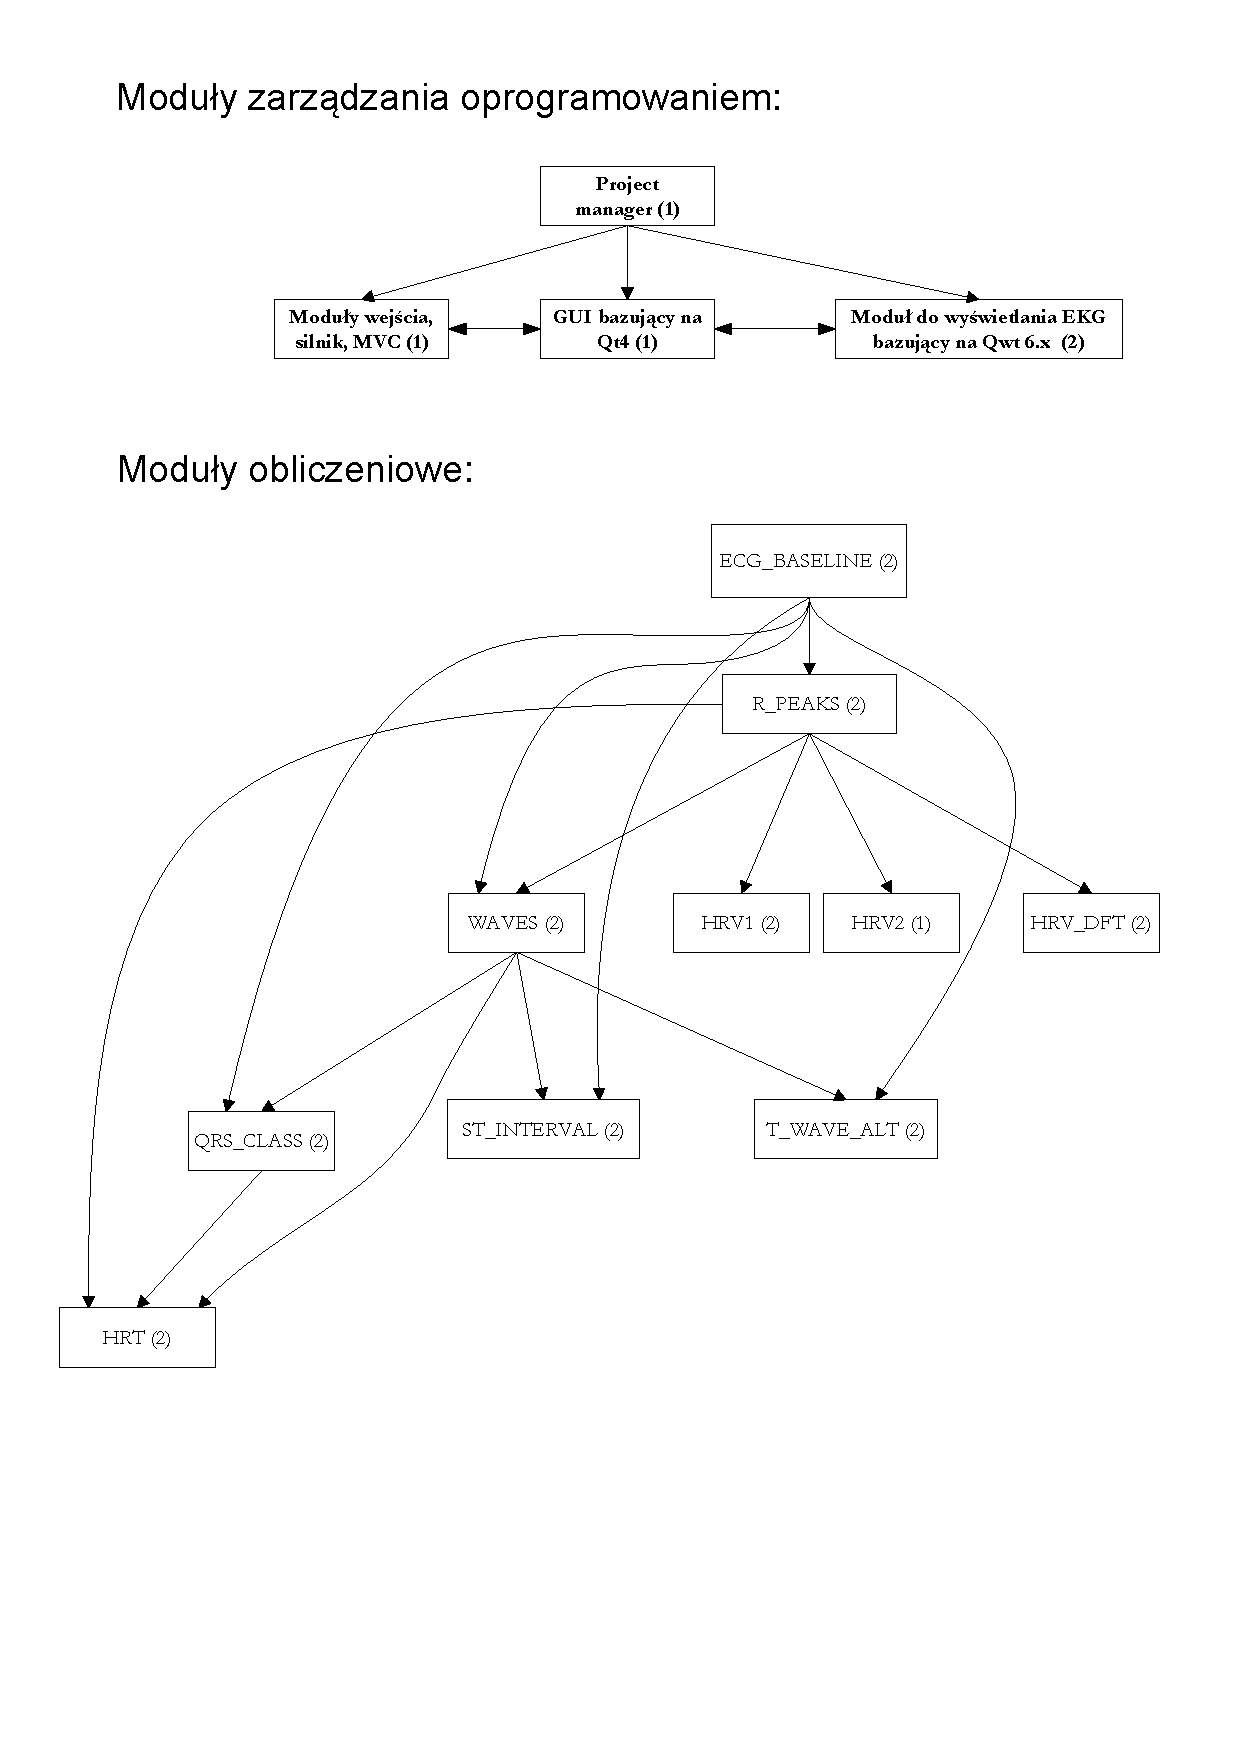
\includegraphics[width=0.7\linewidth]{include/Projekt_zaleznosci}
  \label{fig:zaleznosci}
  \caption{Zależności pomiędzy modułami projektu.}
\end{figure}

\section{Specyfikacja techniczna rozwiązania}
\label{sec:techspec}

\subsection{Wykorzystane narzędzia}
\label{sec:tools}

Podczas realizacji projektu wykorzystywane były różne narzędzia do tworzenia i prototypowania rozwiązań. Wstępne projekty przygotowywane były w programie Matlab, zaś ostateczny kod powstawał w języku C++ (standard '03 z elementami standardu C++11 obsługiwanymi przez wspierane kompilatory).
Minimalne wymagania kompilacji projektu są następujące:
\begin{itemize}
  \item Jeden z kompilatorów:
  \begin{itemize}
    \item Microsoft Visual Studio 2010
    \item GCC 4.5
  \end{itemize}
  \item Biblioteki:
  \begin{itemize}
    \item Boost 1.51
    \item Qt 4.8
    \item Qwt 6.01
    \item gsl 1.15
    \item WFDB 10.5.16 (zawarta w źródłach projektu)
    \item FFTW 3.3.2
  \end{itemize}
\end{itemize}

Do wersjonowania i śledzenia błędów wykorzystywaliśmy platformę Github wraz z rozproszonym systemem kontroli wersji Git. Posiada on zaawansowane możliwości wspierające pracę grupową nad projektem, co szczególnie przydaje się, gdy liczba osób jest duża.

\subsection{Projekt systemu}
\label{sec:sys_proj}

Program został wykonany w architekturze MVC -- istnieje ścisły podział na część wyświetlającą interfejs użytkownika, moduły przetwarzania sygnału oraz kontroler łączący te dwa elementy, co obrazuje diagram pakietów \ref{fig:package_diagram}. Zastosowano obiektowe podejście przy projektowaniu hierarchii klas realizujących przetwarzanie (rys. \ref{fig:class_diagram}), umożliwiające bezproblemową wymianę implementacji dowolnego modułu na inną.

\begin{figure}[h!]
  \centering
  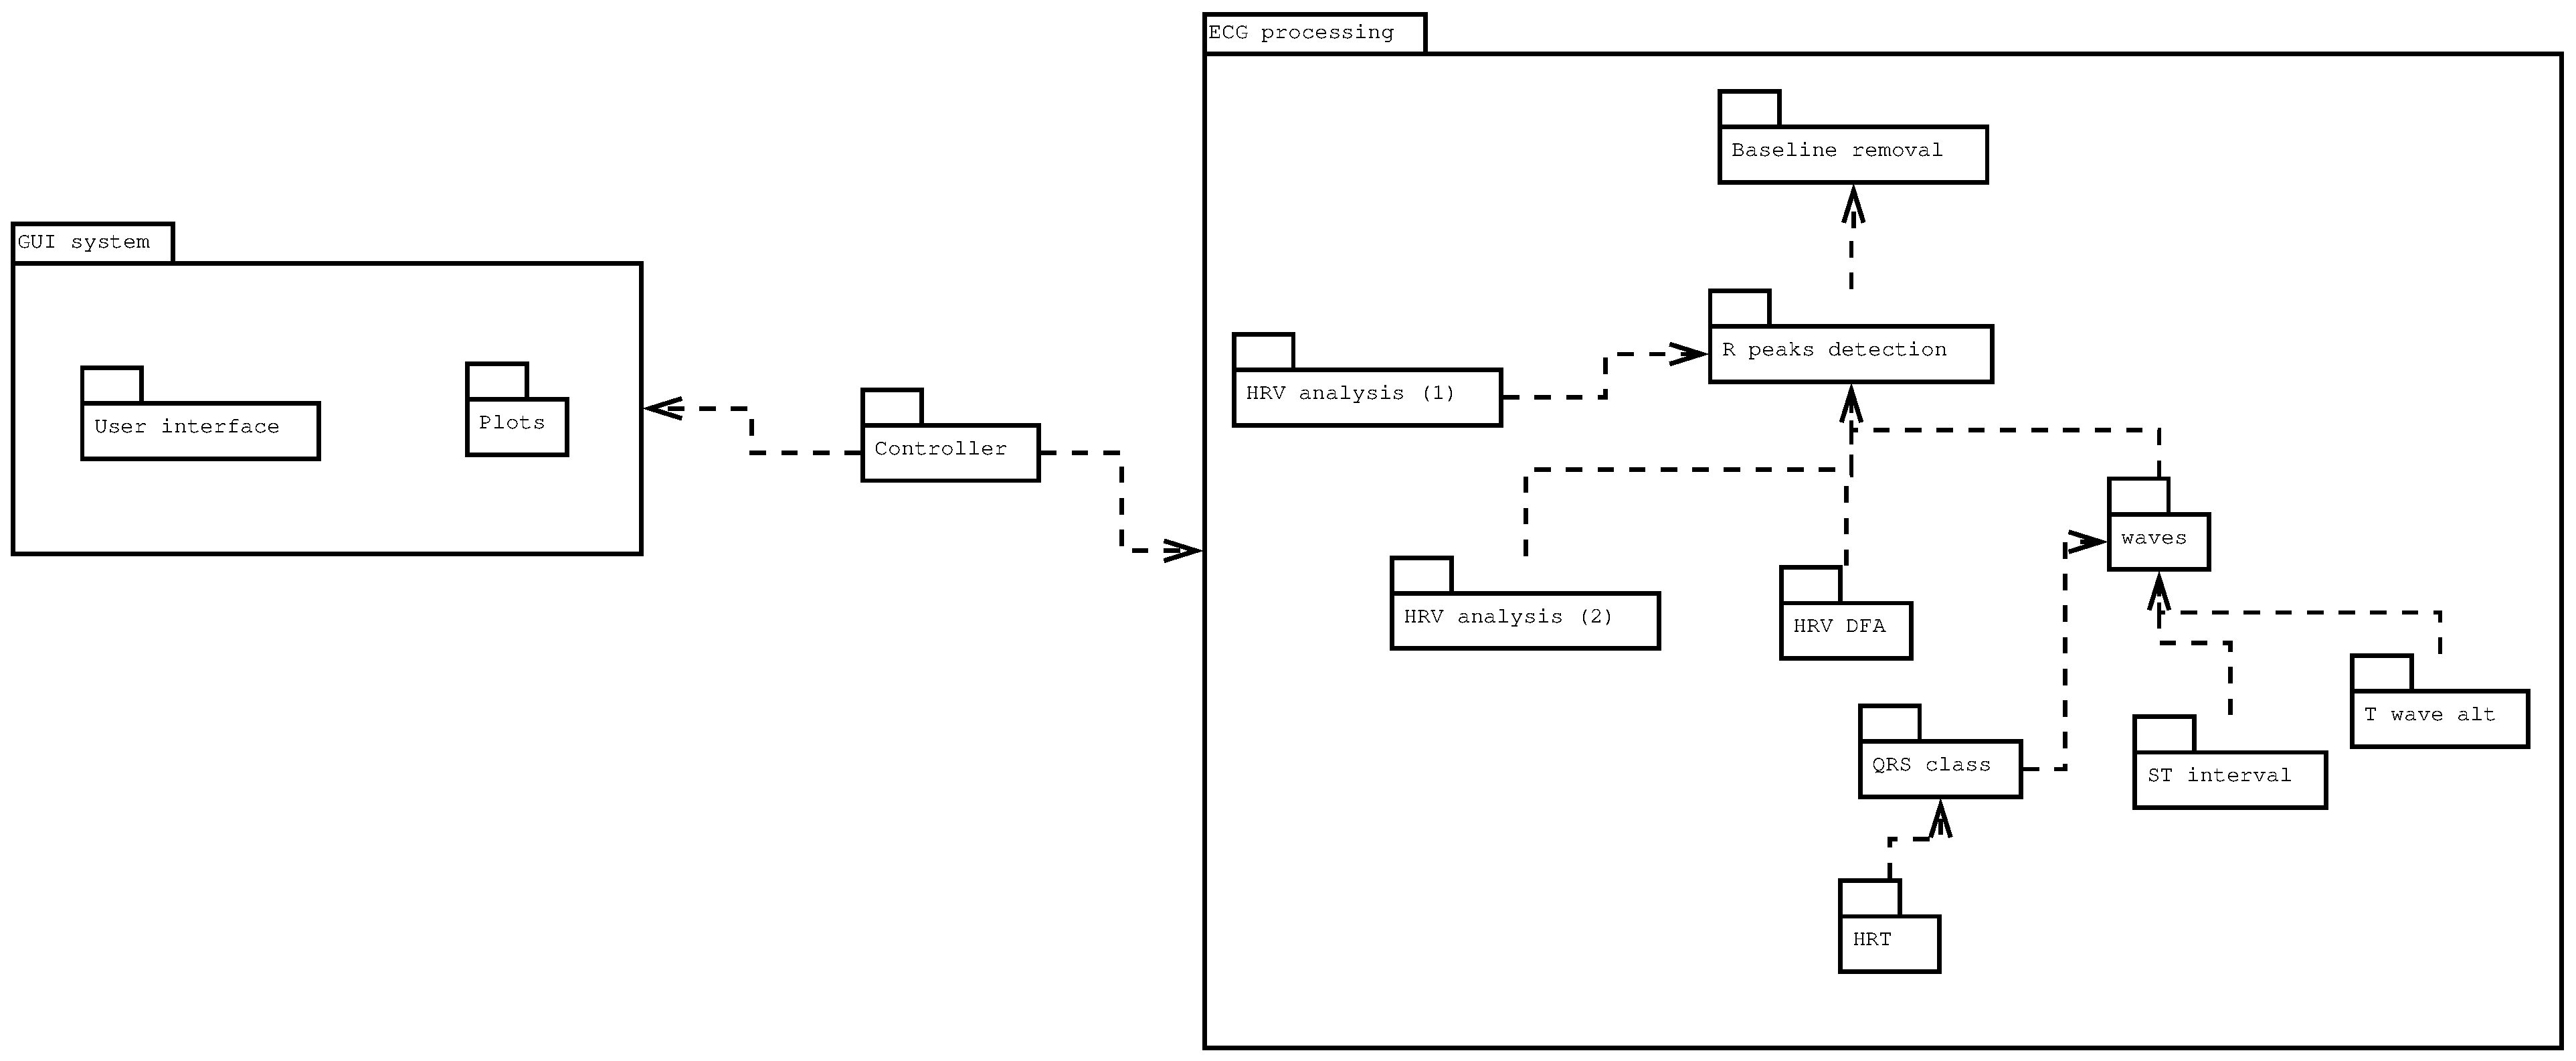
\includegraphics[width=\linewidth]{include/package_diagram}
  \label{fig:package_diagram}
  \caption{Diagram pakietów.}
\end{figure}

Samo przetwarzanie realizowane jest wielofazowo -- moduły przeliczane są sekwencyjnie na osobnym wątku niż wątek zdarzeń GUI, co pozwala na zatrzymanie zbyt długo trwającej operacji. Zaimplementowano także mechanizm buforowania wyników, dzięki czemu przy zmianie parametrów pewnego modułu nie ma konieczności przeliczania wyników modułów wcześniejszych.

Cała aplikacja napisana jest jako samodzielny, wieloplatformowy program (rys. \ref{fig:deployment_diagram}) -- możliwa jest kompilacja pliku binarnego pod systemami Windows, Linux i MacOS X. Całe przetwarzanie wykonywane jest lokalnie, dzięki czemu nie jest wymagane połączenie z Internetem. Dzięki wybraniu licencji GPL v2+ projekt jest wolny i możliwy jest jego dalszy rozwój i kompilacja na nowe platformy.

\begin{figure}[h!]
  \centering
  \includegraphics[width=0.5\linewidth]{include/deployment_diagram}
  \label{fig:deployment_diagram}
  \caption{Diagram wdrożenia.}
\end{figure}

\section{Opisy modułów}
\label{sec:mod}

\subsection{Usuwanie linii bazowej}
\label{sec:baseline}
Autorzy: Weronika Łabaj i Piotr Matuszkiewicz.

\subsubsection{Opis zadania}
\label{sec:baseline:desc}

\begin{description}
\item[Temat] Metody filtracji i detekcji izolinii w sygnale EKG
\item[Opis] Występujące zakłócenia sieciowe i mięśniowe, jak również falowanie linii izoelektrycznej w sygnale EKG niejednokrotnie uniemożliwiają właściwą i poprawną analizę sygnału. Celem projektu jest opracowanie i implementacja metod związanych filtracją i detekcją linii izoelektrycznej w sygnale EKG. W szczególności należy rozważyć:
  \begin{itemize}
  \item filtr Butterwortha,
  \item średnią kroczącą,
  \item metody nieadaptacyjne: filtr Savitzky-Golay’a
  \item metody atapdacyjne np. filtr Wienera, LMS
  \end{itemize}
\item[Dane] ciąg próbek sygnału EKG z bazy Physionet.org
\item[Szukane] moduł programu filtrujący sygnał EKG z zakłóceń sieciowych/mięśniowych oraz usuwający z sygnału falowanie linii izoelektrycznej przy wykorzystaniu różnych metod; w ostatecznym module programu będzie możliwość wyboru algorytmu filtrującego i usuwającego falowanie linii izoelektrycznej
\end{description}

\subsubsection{Badania literaturowe}
\label{sec:baseline:papers}

\subsubsection{Opis procedur i metod}
\label{sec:baseline:procs}

\subsubsection{Warunki testowania}
\label{sec:baseline:tests}

\subsubsection{Wyniki}
\label{sec:baseline:results}

\subsection{Wykrywanie załamków R}
\label{sec:Rs}

\subsection{Waves}
\label{sec:waves}

\subsection{HRV1}
\label{sec:hrv1}

\subsection{HRV2}
\label{sec:hrv2}

Autor: Krzysztof Farganus


\subsubsection{Opis zadania}
\label{sec:hrv2:desc}

Celem projektu jest opracowanie i implementacja metod geometrycznych
analizy HRV.

Dane przyjmowane przez moduł: 
\begin{itemize}
\item ciąg próbek załamków R z modułu R\_PEAKS.
\end{itemize}
Dane zwracane przez moduł:
\begin{itemize}
\item wykres histogramu 
\item wskaźnik TINN 
\item Indeks Trójkątny
\item wykres Poincare wraz z parametrami SD1 i SD2
\end{itemize}

\subsubsection{Badania literaturowe}
\label{sec:hrv2:papers}

Techniki geometryczne służą do przedstawienia długookresowej zmienności
rytmu serca \cite{hrv2-pl}. Są łatwe do uzyskania, ponieważ bazują na aproksymacji
histogramu trójkątem. Szerokość przedziałów klasowych histogramu ma
tutaj kluczowe znaczenie, gdyż jej wartość wpływa na rezultaty metod
geometrycznych. Głównie stosowany jest zakres wynoszący 7.8125 ms
(1/128 s). Powodem jest częstotliwość próbkowania sygnału o najczęściej
występującej wartości 128 Hz.

Cechy metod geometrycznych: 
\begin{itemize}
\item odporność na zakłócenia ze względu na zastosowanie technik aproksymacyjnych
\item eliminacja artefaktów zlokalizowanych poza trójkątem 
\item wyniki niezależne od jakości zapisu sygnału 
\item rezultaty zależne od czasu rejestracji 
\item wymagana duża liczba odstępów RR dla poprawnej analizy (minimalny
czas zapisu \textendash{} 20 minut) 
\end{itemize}
Do najbardziej rozpowszechnionych metod należą: 
\begin{itemize}
\item Wykres histogramu przedstawiający rozkład interwałów RR
\item Indeks trójkątny (HRV triangular index ) - całkowita liczba wszystkich
odstępów RR podzielona przez liczbę odstępów RR o najczęściej spotykanym
czasie trwania. 
\item Trójkątna interpolacja odstępów RR (TINN) \textendash{} długość podstawy
trójkąta aproksymującego histogram kolejnych odstępów interwałów RR
rytmu zatokowego wyrażana w milisekundach. 
\item Wykres Poincare - graficzna reprezentacja korelacji pomiędzy kolejnymi
interwałami , gdzie każdy odstęp RR jest opisany funkcją RR+1. Do
analizy rozproszenia punktów na wykresie stosuje się dwa deskryptory:
SD1 oraz SD2, odpowiadające odchyleniom standardowym. Pierwszy charakteryzuje
rozkład punktów w poprzek linii identyczności, natomiast drugi wzdłuż
tej linii.
\end{itemize}
\textbf{Algorytm obliczania wskaźnika TINN \cite{hrv2-eng}}

Aby obliczyć parametr TINN, czyli wyznaczyć wartości punktów N i M
należy opracować funkcję multiliniową q(t) o postaci:
\begin{itemize}
\item $q(t) = 0$ dla \ensuremath{t \le N}
\item $q(t) = 0$ dla \ensuremath{t \ge M} 
\item $q(X) = Y$ w pozostałych przypadkach
\end{itemize}
a następnie znaleźć minimum z całki o wzorze:

\begin{equation}
\int_{0}^{+\infty}\left(\: D(t)\right)-q(t)\:)^{2}dt
\end{equation}

spośród wszystkich kombinacji punktów (N,M) , gdzie D(t) to wartość
histogramu. W układzie dyskretnym poprzedni wzór wygląda następująco:

\begin{equation}
\sum(\: D(t)-q(t)\:)^{2}\rightarrow \text{minimum}
\end{equation}


przy czym dla $t\:\epsilon(0,N)$ oraz $t\:\epsilon(M,\infty)$ ma
postać: 

\begin{equation}
D(t)^{2}
\end{equation}


natomiast dla $t\:\epsilon\left\langle 0,N\right\rangle$ wygląda
następująco: 
\begin{equation}
(D(t)-q(t))^{2}
\end{equation}

Algorytm obliczania parametrów SD1 i SD2

Parametry SD1 i SD2 są wyznaczane według poniższych wzorów:

\begin{align}
SD1 &= \sqrt{\frac{1}{2}\cdot SDSD^{2}} \\
SD2 &= \sqrt{2\cdot SDNN^{2}-\frac{1}{2}\cdot SDSD^{2}}
\end{align}


gdzie:
\begin{itemize}
\item SDNN to odchylenie standardowe interwałów RR: $SDNN=\sqrt{\frac{1}{N-1}\cdot\sum_{i=1}^{N}\left(\bar{RR}-RR_{i}\right)^{2}}$
\item SDSD to odchylenie standardowe różnic pomiędzy dwoma sąsiadującymi
interwałami: $SDSD=\sqrt{E\left\{ \triangle RR_{j}^{2}\right\} -E\left\{ \triangle RR_{j}\right\} ^{2}}$
\end{itemize}

\subsubsection{Opis procedur i metod }
\label{sec:hrv2:procs}

\paragraph{\texttt{GeometricAnalysis::runModule}} -- wirtualna funkcja uruchamiająca moduł HRV2.

\medskip{}


Argumenty funkcji:
\begin{itemize}
\item \verb+ECGInfo info+ -- dane o wczytanym sygnale
\item \verb+ECGRs ecgRs+ -- wektor numerów próbek zawierający załamki R
\item \verb+ECGHRV2 ecgHRV2+ -- instancja klasy przechowującej wyniki analizy zmienności
rytmu serca metodami geometrycznymi
\end{itemize}
\medskip{}


Funkcja zwraca:

Funkcja przekazuje wyniki metod geometrycznych analizy HRV do instancji
klasy \verb+ECGHRV2+.

\medskip{}


Używane funkcje:
\begin{itemize}
\item \verb+PrepareRRSignal+
\item \verb+MakeHistogramAndGeometricalParams+
\item \verb+MakePoincareAndSDParams+
\item \verb+SetHRV2Params+\medskip{}

\end{itemize}
Używane zmienne:
\begin{itemize}
\item \verb+ECGRs rpeaks+ -- atrybut klasy \verb+GeometricAnalysis+ przechowujący wektor
numerów próbek z załamkami R
\item \verb+double SamplingInterval+ -- atrybut klasy \verb+GeometricAnalysis+ przechowujący
częstotliwość wczytanego sygnału
\end{itemize}


\medskip{}

\paragraph{\texttt{GeometricAnalysis::PrepareRRSignal}} -- funkcja przekształca wektor numerów próbek z załamkami R na wektor
interwałów RR w milisekundach.

\medskip{}


Argumenty funkcji:
\begin{itemize}
\item \verb+rpeaks+ -- wektor numerów próbek z załamkami R
\end{itemize}
\medskip{}


Funkcja zwraca:

Funkcja zapisuje wektor interwałów RR w atrybucie klasy \verb+RR_intervals+.

\medskip{}


Używane funkcje:
\begin{itemize}
\item \verb+gsl_vector_int_get+ -- metoda GSL pobierająca całkowitą wartość danego
elementu z wektora
\item \verb+gsl_vector_set+ -- metoda GSL zapisująca zmiennoprzecinkową wartość
w danym elemencie wektora
\item \verb+gsl_vector_scale+ -- metoda GSL mnożąca każdy element wektoru przez
liczbę zmiennoprzecinkową
\end{itemize}
\medskip{}


Używane zmienne:
\begin{itemize}
\item \verb+unsigned int rpeaks_size+ -- długość wektora z numerami próbek załamków
R
\item \verb+double SamplingInterval+ -- częstotliwość wczytanego sygnału
\end{itemize}

\medskip{}

\paragraph{\texttt{GeometricAnalysis::MakeHistogramAndGeometricalParams}} -- funkcja tworzy wektor wartości histogramu, oblicza wysokość i pozycję
kolumny histogramu reprezentującą najczęściej powtarzający się interwał
RR, wylicza długość oraz pozycję podstawy trójkąta aproksymującego,
oszacowuje wartość indeksu trójkątnego.

\medskip{}


Argumenty funkcji:
\begin{itemize}
\item \verb+RR_intervals+ -- wektor interwałów RR w milisekundach
\end{itemize}
\medskip{}


Funkcja zwraca:
\begin{itemize}
\item histogram\_x -- pozycje kolumn histogramu
\item histogram\_y -- wysokości kolumn histogramu
\item X -- pozycja najwyższej kolumny histogramu
\item Y -- wysokość najwyższej kolumny histogramu
\item N -- początek podstawy trójkąta aproksymującego
\item M -- koniec podstawy trójkąta aproksymującego
\item HRVTriangularIndex -- indeks trójkątny
\item TINN -- wskaźnik TINN
\end{itemize}
\medskip{}


Używane funkcje:
\begin{itemize}
\item \verb+gsl_vector_max+ -- metoda GSL zwracająca największy element danego
wektora
\item \verb+gsl_vector_min+ -- metoda GSL zwracająca najmniejszy element danego
wektora
\item \verb+gsl_vector_int_max_index+ -- metoda GSL zwracająca pozycję największego
elementu danego wektora
\item \verb+gsl_vector_int_get+ -- metoda GSL pobierająca całkowitą wartość danego
elementu z wektora
\item \verb+gsl_vector_get+ -- metoda GSL pobierająca zmiennoprzecinkową wartość
danego elementu z wektora
\item \verb+gsl_vector_set+ -- metoda GSL zapisująca zmiennoprzecinkową wartość
w danym elemencie wektora
\item \verb+gsl_vector_int_set+ -- metoda GSL zapisująca całkowitą wartość w
danym elemencie wektora
\item \verb+gsl_interp_alloc+ -- metoda GSL tworząca wskaźnik do nowo utworzonego
obiektu interpolacji
\item \verb+gsl_interp_accel_alloc+ -- metoda GSL tworząca wskaźnik na obiekt
iteratora do wyszukiwania interpolacji 
\item \verb+gsl_interp_init+ -- metoda GSL wyliczająca funkcję interpolującą
\item \verb+gsl_interp_eval+ -- metoda GSL zwracająca punkt funkcji interpolującej 
\end{itemize}
\medskip{}


Używane zmienne:
\begin{itemize}
\item \verb+double RRmax+ -- najdłuższy interwał RR
\item \verb+double RRmin+ -- najkrótszy interwał RR
\item \verb+IntSignal Histogram+ -- tymczasowy wektor punktów histogramu
\item \verb+unsigned Histogram_size+ -- liczba wszystkich kolumn histogramu
\item \verb+unsigned int RR_intervals_size+ -- liczba wszystkich interwałów RR
\item \verb+double minimum+ -- zmienna przechowująca minimalną wartość całki z algorytmu
wyznaczania TINN
\item \verb+double x[3], y[3]+ -- tablica współrzędnych trójkąta aproksymującego
\end{itemize}


\paragraph{\texttt{GeometricAnalysis::MakePoincareAndSDParams}} -- funkcja wylicza punkty wykresu Poincare oraz parametry: SD1 i SD2.

\medskip{}


Argumenty funkcji:
\begin{itemize}
\item \verb+RR_intervals+ -- wektor interwałów RR w milisekundach
\end{itemize}
\medskip{}


Funkcja zwraca:
\begin{itemize}
\item poincare\_x -- współrzędne osi OX wykresu Poincare
\item poincare\_y -- współrzędne osi OY wykresu Poincare
\item parametr SD1
\item parametr SD2
\end{itemize}
\medskip{}


Używane funkcje:
\begin{itemize}
\item \verb+gsl_vector_get+ -- metoda GSL pobierająca zmiennoprzecinkową wartość
danego elementu z wektora
\item \verb+gsl_vector_int_set+ -- metoda GSL zapisująca całkowitą wartość w
danym elemencie wektora
\item \verb+gsl_stats_sd+ -- metoda GSL wyliczająca odchylenie standardowe
\item \verb+gsl_vector_int_sub+ -- metoda GSL odejmująca dwa wektory
\end{itemize}
\medskip{}


Używane zmienne:
\begin{itemize}
\item \verb+unsigned int RR_intervals_size+ -- liczba wszystkich interwałów RR
\item \verb+IntSignal diff+ -- wektor różnic pomiędzy sąsiednimi interwałami RR
\end{itemize}
%

\paragraph{\texttt{GeometricAnalysis::SetHRV2Params}} -- funkcja przekazuje wyniki analizy HRV metodami geometrycznymi do instancji
klasy ECGHRV2.

\medskip{}


Argumenty funkcji:
\begin{itemize}
\item \verb+ECGHRV2 &hrv2+
\end{itemize}
\medskip{}


Funkcja zwraca:

Funkcja zwraca wyniki analizy geometrycznej do \verb+ECGHRV2 &hrv2+.

\medskip{}


Używane funkcje:
\begin{itemize}
\item wszystkie funkcje pozwalające na zapis wyników do atrybutów klasy
ECGHRV2. \medskip{}

\end{itemize}
Używane zmienne:

Funkcja nie używa dodatkowych zmiennych.%


\paragraph{\texttt{GeometricAnalysis::MakeRRsignal}} -- funkcja tworząca testowy wektor interwałów RR w milisekundach.

\medskip{}


Argumenty funkcji:

Nie przyjmuje argumentów.

\medskip{}


Funkcja zwraca:

Funkcja zwraca testowy wektor interwałów RR jako instancję klasy ECGRs.

\medskip{}


Używane funkcje:
\begin{itemize}
\item \verb+gsl_vector_int_set+ -- metoda GSL zapisująca całkowitą wartość w
danym elemencie wektora
\item \verb+setRs+ -- zapisuje wektor w instancji klasy ECGRs
\end{itemize}
\medskip{}


Używane zmienne:
\begin{itemize}
\item \verb+int RRsignal_length+ -- długość wektora interwałów RR
\item \verb+int RRsignal[]+ -- tablica wartości interwałów RR
\end{itemize}
%

\paragraph{\texttt{GeometricAnalysis::setParams}} -- funkcja modyfikująca szerokość kolumny histogramu.

\medskip{}


Argumenty funkcji:
\begin{itemize}
\item \verb+ParametersTypes &parameterTypes+ -- zawiera dane ustawień poszczególnych
modułów
\end{itemize}
\medskip{}


Funkcja zwraca:

Nie zwraca niczego. 

\medskip{}


Używane funkcje:
\begin{itemize}
\item \verb+parameterTypes.find(histogram_bin_length)+
- wyszukuje parametr modyfikujący szerokość kolumny histogramu\medskip{}

\end{itemize}
Używane zmienne:
\begin{itemize}
\item \verb+double HistogramParameter+ -- zmienna przechowująca rezultat funkcji \verb+parameterTypes.find+.
\item \verb+double HistogramBinLength+ -- atrybut klasy \verb+GeometricAnalysis+ przechowujący
szerokość kolumny histogramu.
\end{itemize}


\subsubsection{Warunki Testowania}
\label{sec:hrv2:tests}

Podczas procesu implementacji, moduł HRV2 poddawany był dwóm rodzajom
testów:
\begin{itemize}
\item Pierwszy test polegał na porównaniu wyników działania modułu zaimplementowanego
w Matlabie oraz Visual Studio Ultimate 2010. W tym celu jako dane
wejściowe wykorzystano wektor interwałów RR wczytywany z pliku tekstowego
dla Matlaba z tablicy jednowymiarowej dla Visual Studio.
\item Drugi test sprawdzał działanie programu, gdy ten korzystał z testowych
wyników modułu R\_PEAKS.
\end{itemize}

\subsubsection{Wyniki}
\label{sec:hrv2:results}

Rysunki \ref{fig:hrv2_1}, \ref{fig:hrv2_2} oraz \ref{fig:hrv2_3} prezentują wyniki pierwszego testu opisanego w poprzedniej
podsekcji:

\begin{center}
%
\begin{figure}
\begin{centering}
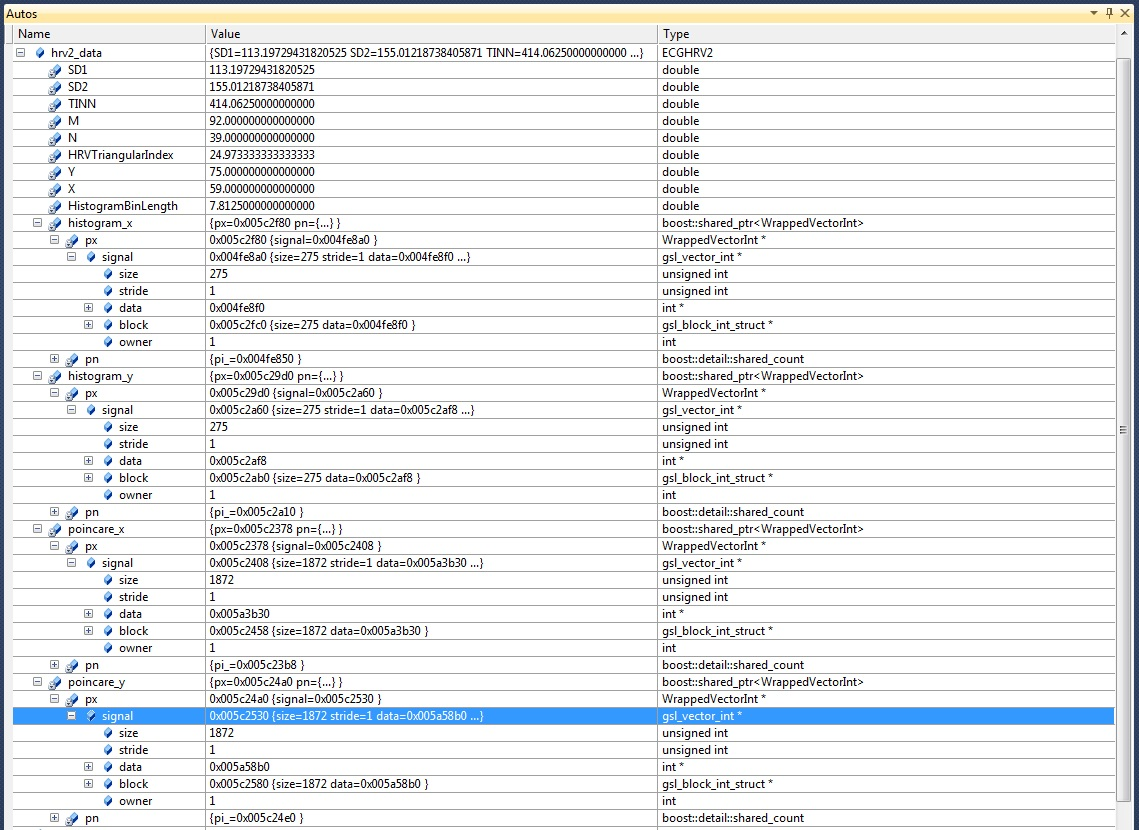
\includegraphics[scale=0.4]{include/hrv2_1}
\par\end{centering}

\caption{Wyniki modułu HRV2 -- Visual Studio Ultimate 2010}
\label{fig:hrv2_1}
\end{figure}

\par\end{center}

\begin{center}
%
\begin{figure}
\begin{centering}
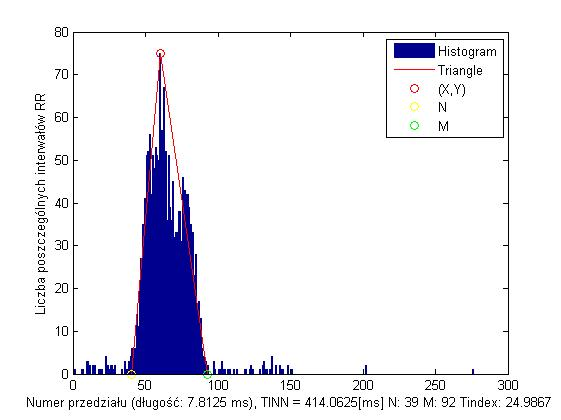
\includegraphics[scale=0.7]{include/hrv2_2}
\par\end{centering}

\caption{Wykres histogramu -- Matlab}
\label{fig:hrv2_2}
\end{figure}

\par\end{center}

\begin{center}
%
\begin{figure}
\begin{centering}
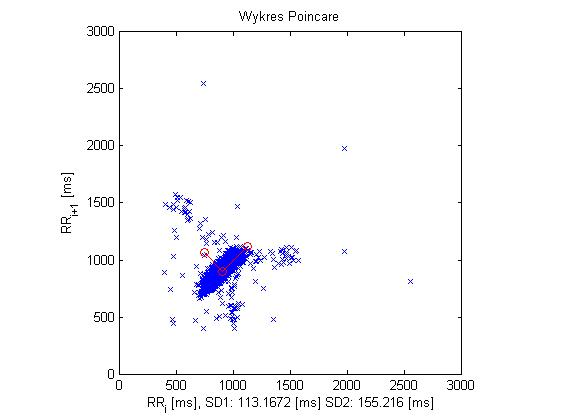
\includegraphics[scale=0.7]{include/hrv2_3}
\par\end{centering}

\caption{Wykres Poincare -- Matlab}
\label{fig:hrv2_3}
\end{figure}

\par\end{center}

\subsection{HRV DFA}
\label{sec:hrvd_fa}

\subsection{Klasyfikacja zespołów QRS}
\label{sec:qrs_class}
Autorzy: Krzysztof Bębenek

\subsubsection{Opis zadania}
\label{sec:qrs_class:desc}

\begin{description}
\item[Temat] Metody detekcji morfologicznego pochodzenia zespołu QRS.
\item[Opis] Proces automatycznego klasyfikowania zespołów QRS należy do jednego z trudniejszych procesów podczas przetwarzania sygnałów EKG. Jest jednak on niezbędny w dalszych etapach analizy podczas których brane są pod uwagę tylko niepoprawne pobudzenia. Do prostych sposób oceny morfologi pobudzenia służą:
  \begin{itemize}
  \item współczynnik kształtu Malinowskiej,
  \item stosunek części ujemnej do dodatniej sygnału,
  \end{itemize}
\item[Dane] ciąg próbek przefiltrowanego sygnału EKG, wektory QRS\_onset oraz QRS\_end określające początek oraz koniec zespołu QRS
\item[Szukane] moduł programu klasyfikujący zespołu QRS na podstawie ich morfologii 
\end{description}

\subsubsection{Badania literaturowe}
\label{sec:qrs_class:papers}

\subsubsection{Opis procedur i metod}
\label{sec:qrs_class:procs}

\subsubsection{Warunki testowania}
\label{sec:qrs_class:tests}

\subsubsection{Wyniki}
\label{sec:qrs_class:results}



\subsection{ST interval}
\label{sec:st_interval}
Autorzy: Bartłomiej Bułat i Krzysztof Piekutowski.

\subsubsection{Opis zadania}
\label{sec:st_interval:desc}
Celem projektu jest wyznaczenie odcinków ST, pomiar poziomu odcinka ST względem linii izoelektrycznej i jego nachylenia, a także detekcja epizodów ST oraz parametry ilościowe i jakościowe epizodów ST. Celowość analizy odcinka ST względem linii izoelektrycznej związana jest z predykcją choroby wieńcowej, miażdżycy oraz niedotlenieniem mięśnia serca.

Dane przyjmowane przez moduł:
\begin{itemize}
  \item sygnał ECG\_BASELINE;
  \item wektor numerów próbek załamków R z modułu R PEAKS;
  \item wektor numerów próbek punktów charakterystycznych z modułu WAVES:
  \begin{itemize}
    \item $QRS_{onset}$
    \item $QRS_{end}$
    \item $T_{end}$
  \end{itemize}  
\end{itemize}

Dane zwracane przez moduł:
\begin{itemize}
  \item wektor wykrytych odcinków ST zawierających informaje:
  \begin{itemize}
    \item początek i koniec odcinka;
    \item poziom izolinii;
    \item pomiar poziomu względem izolinii;
    \item pomiar nachylenia odcinka ST;
    \item opis słowny interwału;
  \end{itemize}
  \item wektor wykrytych epizodów wraz z parametrami:
  \begin{itemize}
    \item numer próbki początku epizodu;
    \item numer próbki końca epizodu.
  \end{itemize}
\end{itemize}

\subsubsection{Badania literaturowe}
\label{sec:st_interval:papers}

\subsubsection{Opis procedur i metod}
\label{sec:st_interval:procs}

Główna funkcjonalność modułu znajduje się w klasie \verb|STAnalysis|. Klasa ta,
według przyjętego schematu rozszerza abstrakcyjny moduł analizy odcinka ST. W
tej klasie znajdują się drzewo klas prywatnych reprezentujących poszczególne
algorytmy analizy. W szczególności dwie klasy \verb|SimpleAnalizer| oraz
\verb|ComplexAnalizer|. Pierwsza klasa reprezentuje najprostszy algorytm
zaprezentowany w \cite[p.~155]{AUGUST1}, druga zaś implementuje lekko
zmodyfikowany algorytm opisany w \cite{SHEN1}.

%% TODO: mienić nazwę funkcji w programie
Lista i opis najważniejszych funkcji:

\begin{lstlisting}
void STAnalysis::SimpleAnalizer::analyse(const int it, const ECGRs& rpeaks,
  const ECGWaves& waves, const ECGSignalChannel& signal,
  const  ECGInfo& info, ECGST& output);
\end{lstlisting}

Funkcja analizująca załamek ST w zespole QRS numer \verb|it|. Wykorzystując
punkty sygnału obliczone we wcześniejszych modułach (tj. $QRS_{onset}$,
$QRS_{end}$ oraz $T_{end}$) oblicza koniec odcinka ST i wylicza jego parametry:
\begin{itemize}
  \item przesunięcie względem izolinii
  \item wartość nachylenia w stosunku do izolini
  \item długość odcinka ST
\end{itemize}
Uzywając wczesniej ustawionego parametru \verb|simple_thresh|, odcinek ST
określany jest jako ,,normalny'', ,,uniesiony'' lub ,,obniżony''.

Parametry:
\begin{itemize}
  \item \verb|const int it| -- numer badanego zespołu QRS, jako liczba
    porządkowa numerów próbek z tablicy załamków R.
  \item \verb|const ECGR& rpeaks| -- struktura zawierająca tablicę numerów
    próbek kolejnych załamków R
  \item \verb|const ECGEaves& waves| -- struktura zawierająca tablice
    przechowujące numery próbek punktów charakterystycznych kolejnych zespołów
    QRS: $P_{onset}$, $QRS_{onset}$, $QRS_{end}$ oraz $T_{end}$.
  \item \verb|const ECGSignalChanel& signal| -- jeden kanał odfiltrowanego
    sygnału z usuniętym przesunięciem izolinii.
  \item \verb|const ECGInfo& info| -- struktura zawierająca informacje o badanym
    sygnale EKG, m.in. częstotliwość.
  \item \verb|ECGST& output| -- parametr wyjściowy, struktura zawierająca
    tablice wszystkich interwałów ST wraz z ich parametrami, oraz tablice
    zarejestrowanych epizodów ST wraz z ich parametrami.
\end{itemize}

\begin{lstlisting}
void STAnalysis::ComplexAnalizer::analyse(const int it, const ECGRs& rpeaks,
  const ECGWaves& waves, const ECGSignalChannel& signal,
  const  ECGInfo& info, ECGST& output);
\end{lstlisting}

Funkcja analizująca załamek ST w zespole QRS numer \verb|it|. Wykorzystując
punkty sygnału obliczone we wcześniejszych modułach (tj. $QRS_{onset}$,
$QRS_{end}$ oraz $T_{end}$) oblicza koniec odcinka ST (wykorzystując bardziej
zaawansowane algorytmy od poprzedniej funkcji), a następnie oblicza jego parametry:
\begin{itemize}
  \item przesunięcie względem izolinii,
  \item wartość nachylenia w stosunku do izolinii,
  \item długość odcinka ST,
  \item klasyfikacja kształtu.
\end{itemize}
Używając wcześniej ustawionego parametru \verb|complex_thresh|, odcinek ST
określany jest jako ,,normalny'', ,,uniesiony'' lub ,,obniżony''. Algorytm
ocenia również to, czy załamek jest prosty czy zakrzywiony w oparciu o
wcześniej ustawiony parametr \verb|type_thresh|. Dla prostych odcinków określa
kierunek, czy narasta, opada czy jest poziomy. Do określenia tej cechy
wykorzystywany jest parametr \verb|slope_thresh|. Dla zakrzywiony odcinków ST
oceniana jest wypukłość krzywej. Szczegółowy opis działania znajduje się w
poprzednim rozdziale.

Parametry:
\begin{itemize}
  \item \verb|const int it| -- numer badanego zespołu QRS, jako liczba
    porządkowa numerów próbek z tablicy załamków R.
  \item \verb|const ECGR& rpeaks| -- struktura zawierająca tablicę numerów
    próbek kolejnych załamków R
  \item \verb|const ECGEaves& waves| -- struktura zawierające tablice
    przechowujące numery próbek punktów charakterystycznych kolejnych zespołów
    QRS: $P_{onset}$, $QRS_{onset}$, $QRS_{end}$ oraz $T_{end}$.
  \item \verb|const ECGSignalChanel& signal| -- jeden kanał odfiltrowanego
    sygnału z usuniętym przesunięciem izolinii.
  \item \verb|const ECGInfo& info| -- struktura zawierająca informacje o badanym
    sygnale EKG, m.in. częstotliwość.
  \item \verb|ECGST& output| -- parametr wyjściowy, struktura zawierająca
    tablice wszystkich interwałów ST wraz z ich parametrami, oraz tablice
    zarejestrowanych epizodów ST wraz z ich parametrami.
\end{itemize}

Funkcje pomocnicze klasy \verb|ComplexAnalizer|:

\begin{lstlisting}
int STAnalysis::ComplexAnalizer::getTPeak(const OtherSignal& sig,
  int from, int to);
\end{lstlisting}

Funkcja wyszukująca położenia punktu $T_{peak}$ na zadanym odcinku sygnału.
Początkiem wyszukiwania szczytu fali T jest zwykle punkt 20ms za punktem
$QRS_{end}$, a punktem końcowym jest koniec fali T. Funkcja wykorzystuje
dyskretną pochodną sygnału.

Parametry:
\begin{itemize}
  \item \verb|const OtherSignal& sig| - cały, odfiltrowany sygnał EKG
  \item \verb|int from| - numer próbki w której należy zacząć poszukiwania
  \item \verb|int to| - numer próbki w której należy skończyć poszukiwania
\end{itemize}


\begin{lstlisting}
std::pair<int, double> maxDistanceSample(const OtherSignal& signal, 
  int from, int to);
\end{lstlisting}

Funkcja szukająca numeru próbki najbardziej oddalonego od liniowej interpolacji
fragmentu sygnału miedzy dwoma punktami. Oprócz numeru próbki od początku
sygnału, zwracana jest wartość największej różnicy miedzy punktem sygnału, a
prostą interpolacji.

Parametry:
\begin{itemize}
  \item \verb|const OtherSignal& signal| - badany sygnał
  \item \verb|int from| - numer próbki będącej początkiem interesującego
    fragmentu sygnału, równocześnie, pierwszy punkt interpolacji liniowej.
  \item \verb|int to| - numer próbki będącej końcem interesującego fragmentu
    sygnału, równocześnie, drugi punkt interpolacji
\end{itemize}

\begin{lstlisting}
std::pair<int, int> overBelowSamples(const OtherSignal& signal,
  int from, int to);
\end{lstlisting}

Funkcja obliczająca ilość próbek ponad i poniżej prostej interpolującej sygnał
miedzy dwoma punktami. Funkcja wykorzystywana jest do określenia wypukłości
odcinka ST.

Parametry:
\begin{itemize}
  \item \verb|const OtherSignal& signal| - badany sygnał
  \item \verb|int from| - numer próbki będącej początkiem interesującego
    fragmentu sygnału, równocześnie, pierwszy punkt interpolacji liniowej.
  \item \verb|int to| - numer próbki będącej końcem interesującego fragmentu
    sygnału, równocześnie, drugi punkt interpolacji
\end{itemize}

\subsubsection{Warunki testowania}
\label{sec:st_interval:tests}

\subsubsection{Wyniki}
\label{sec:st_interval:results}

\subsection{T wave alt}
\label{sec:t_wave_alt}

\subsection{HRT}
\label{sec:hrt}

\bibliographystyle{plain}
\bibliography{report}
\end{document}
